\section{Optimizing Pointwise Convolution}
\label{sec:pwconv} 
In this section, we explain the workflow of our dynamic tile size scheme for pointwise convolution. \RV{This approach
extends the optimization for convolution operations in our prior work \cite{lu2020optimizing} to pointwise convolution}. Our approach
consists of three stages, described as follows.

In the first and second stages, we identify parameters related to the tile size and determine candidate values for each parameter (Section \ref{sec:pwinputdependent} and Section \ref{sec:pwinputindependent}). The first and second stages process input dependent and independent parameters respectively. In the third
stage, as detailed in Algorithm \ref{algo:pwalgo}, we iterate over all combinations of parameters and search for the combination that
achieves optimal SM utilization and data reuse (Section \ref{sec:searchoptimal}).

We note that previous studies \cite{tanner2018tensile, kelefouras2016high, abdelfattah2019fast, kurzak2015implementation,
jiang2020enabling, tillet2017input, lan2019feathercnn,zhang2012autogeneration} have exploited tiling and autotuning for convolution and
GEMM operations. However, these prior methods are inadequate for pointwise convolutions on GPUs due to two main drawbacks: they do not
consider SM utilization when choosing the optimal tile size and are not designed for pointwise convolutions with small inputs. Our dynamic
tile size scheme avoids these two drawbacks. To improve SM utilization, our approach searches for the optimal tile size for the output
based on the input size to generate a proper number of tiles to saturate GPU and maximize data reuse. To optimize pointwise convolution
with small inputs, we distribute channels across threads within a warp to increase the arithmetic intensity for each thread.


\subsection{Determine Tiling Parameters\label{sec:pwinputdependent}}

In our design, we use a 2-level tiling scheme, as shown in Fig. \ref{fig:pwworkflow}, to partition the output into block tiles and warp tiles.
Each thread block processes one block tile and each warp processes one warp tile.
The height dimension of the warp tile is shared among 32 threads of a warp and the width dimension of the warp tile is distributed across 32 threads of a warp.
Hence, we have two input dependent parameters, namely the height and width of the warp tile, denoted as $Warp_H$ and $Warp_W$ respectively.
Now we introduce how to use the 2-level tiling scheme to determine candidate values for $Warp_H$ and $Warp_W$.
\subsubsection{2-level tiling scheme}
To divide the output into block tiles, we utilize two logical layouts of the output, \textbf{\emph{L1}} and \textbf{\emph{L2}}, as shown in Fig. \ref{fig:pwworkflow}.
$F_N$ and $I_N \times I_H \times I_W$ represent the filter and input dimensions of the output respectively. \RV{Notice that our 2-level tiling can handle arbitrary input sizes since we do not require $I_H = I_W$.}
Before partitioning the output, we first select the layout of the output based on the size of the filter dimension.
The rationale behind choosing the filter dimension instead of the input dimension can be described as follows.
The number of filters, $F_N$, is fixed once the structure of a CNN is determined.
But the size of the input dimension will be affected by the batch size, $I_N$, during inference and training.
Therefore, it is easier to design our approach based on the size of the filter dimension.
When $F_N > 48$, we choose layout \textbf{\emph{L1}} and distribute filter channels across threads within a warp.
Otherwise, we choose layout \textbf{\emph{L2}} and distribute input channels.
The boundary $F_N = 48$ is determined as follows.
Fig. \ref{fig:pwworkflow} demonstrates that in layout \textbf{\emph{L2}}, the maximal value of $F_N$ is $4 \times Warp_H$ and $Warp_H \leq 12$ (explain later in this section), therefore we have $F_N \leq 48$ for layout \textbf{\emph{L2}}.

Since both layouts have the similar procedure, we take layout \textbf{\emph{L1}} as an illustration example and give a brief description of layout \textbf{\emph{L2}} at the end of this section.
After choosing the layout based on $F_N$, we partition the output along the filter dimension.
First, we halve the filter dimension if $F_N \geq 512$.
The reason is that if we let each thread block process a large number of filters, then each thread needs to issue more than 15 global memory load instructions, which may cause MIO (Memory Input Output) instruction queue throttle and leads to performance degradation.
Then, we halve both dimensions of each block tile and generate $2 \times 2$ warp tiles.
\subsubsection{Determine candidates for $Warp_H$ and $Warp_W$}
Based on the partition method, we know that $Warp_W$ can be calculated with $Warp_W=F_N/4$ or $Warp_W=F_N/2$. Thus, we only need to determine candidate values for $Warp_H$ based on the size of the input dimension.
In our design, when $Warp_H > 12$, we need assembly level optimizations like the work in
\cite{yan2020optimizing,yan2020demystifying} for some configurations of pointwise convolutions to avoid register spills. But in this work,
we focus on higher level rather than assembly level optimizations, and thus set $Warp_H \leq 12$.
If the size of the input dimension is large, we prefer to choose a large $Warp_H$ because using small $Warp_H$ will generate many thread blocks and results in multiple loads of shared filters \cite{jia2020enabling, zheng2020flextensor}.
If the size of the input dimension is small, we prefer to choose a small $Warp_H$ because using a large $Warp_H$ will generate a few thread blocks and result in SM underutilization.
Since each thread loads at most 12 input elements ($Warp_H \leq 12$), we set the upper limit of large $Warp_H$ to 12 and the lower limit to $12/2=6$.
Therefore, the candidates for large $Warp_H$ are $Warp_H=\{6,7,8,9,10,11,12\}$.
The candidates for small $Warp_H$ are $Warp_H=\{2,3,4,5,6,7,8\}$.
In our experiments, there is no clear boundary between large and small candidate sets of $Warp_H$, therefore we let both sets overlap in the middle values.
The boundary between the large and small size of the input dimension is experimentally determined as $I_N \times I_H \times I_W=16 \times 14 \times 14$.

Compared to layout \textbf{\emph{L1}}, layout \textbf{\emph{L2}} swaps the input and filter dimensions. Hence, $Warp_H$ can be calculated with $Warp_H=F_N/4$ or $Warp_H=F_N/2$. The candidate values for large $Warp_W$ are $Warp_W=\{6,7,8,9,10,11,12\}$ and for small $Warp_W$ are $Warp_W=\{2,3,4,5,6,7,8\}$.

\subsection{Determine Candidates for Input Independent Parameters\label{sec:pwinputindependent}}

There are three input independent parameters we need to consider, namely the number of warps in a thread block ($Warp_{num}$), the number of thread blocks that can run concurrently on an SM ($Block_{num}$) and the number of channels to be distributed ($C_{num}$).
\subsubsection{Determine candidates for $Warp_{num}$ and $Block_{num}$}
When determining candidates for $Warp_{num}$, we need to consider (1) a small warp number will decrease the opportunity to hide the memory access latency at the warp level, (2) a large warp number will decrease the number of thread blocks and may lead to SM underutilization.
We empirically set the warp number to be four ($Warp_{num}=4$), which gives good performance on our pilot study using microbenchmarks of hand-written pointwise convolution kernels.
For the number of thread blocks, $Block_{num}$, we use two values, 2 and 4, on our evaluation platforms.
These choices are justified as follows. For Nvidia GPUs, each GPU thread can use up to 255 registers, and each SM has 65,536 registers.
If we set $Block_{num}=1$ and $Warp_{num}=4$ (per our discussion above), each SM will have $Block_{num} \times Warp_{num}=4$ wraps.
This allows a thread block to use up to just half of the available registers of an SM because a thread block under this setting can use at most $4\ (warps\ in\ an\ SM) \times 32\ (threads\ per\ warp) \times 255\ (registers\ per\ thread)=32,640$ registers.
Therefore, to utilize the available hardware register, one should set $Block_{num}$ to be greater than one.
We also found that setting $Block_{num}>4$ during searching offers little benefit and hence we set the $Block_{num}$ to be either 2 or 4 ($Block_{num}=\{2,4\}$).

%To achieve the best performance, we iterate over all candidate combinations of $Block_{num}$, $C_{num}$ and $Warp_H$, and select the combination that leads to optimal SM utilization and arithmetic intensity.
\subsubsection{Determine candidates for $C_{num}$\label{sec:cnum}}
When searching for the optimal combination of parameters, a small tile size may be generated, which may lead to low arithmetic intensity and can not hide global memory access latency.
 For example, we assume that the warp tile size is $Warp_H \times Warp_W = 8 \times 64$ and has 56 channels, which means that one warp needs to convolve 8 input elements with 64 filter elements and accumulates results 56 times to generate $8 \times 64=512$ elements. Since the height dimension is shared among 32 threads of the warp, each thread loads 8 input elements, and the width dimension is distributed across 32 threads, each thread loads 2 filter elements. Therefore, each thread accumulates 56 channels of $8 \times 2=16$ elements. Now we can estimate the arithmetic intensity of each thread for one iteration as $\frac{number\ of\ multiplications}{number\ of\ elements}=\frac{8 \times 2}{8 + 2}=1.6$. We can improve arithmetic intensity by distributing channels across threads, as shown in Fig. \ref{fig:pwworkflow}. We distribute eight channels ($C_{num}=8$) of each filter element across 32 threads of the warp.
 In that case, each warp can process $F_{num}=32/C_{num}=32/8=4$ filter elements and each thread processes $T_{num}=Warp_W/F_{num}=64/4=16$ filter elements.
 The arithmetic intensity can be estimated as $\frac{Warp_H \times T_{num}}{Warp_H + T_{num}}=\frac{8 \times 16}{8+16}=5.3$.
 Higher arithmetic intensity increases the chance to hide global memory access latency.
To fully utilize a warp, candidate values for $C_{num}$ should be a power of 2.
Thus, candidates for $C_{num}$ are $C_{num}=\{1,2,4,8,16,32\}$.


\subsection{Search For the Optimal Combination}
\label{sec:searchoptimal}
\subsubsection{Hardware resources constraints}
When searching for the optimal combination of tiling and input independent parameters, we focus on combinations that can meet the hardware resources constraints,
including registers and shared memory. In the rest of this section, we take layout \textbf{\emph{L1}} as an illustration example. Based on
$Block_{num}$, we calculate the number of registers each thread can use ($Limit_R$) and the size of shared memory each thread block can use
($Limit_S$) with formulas $Limit_R=Total_R/(Block_{num}\times Warp_{num} \times 32)$ and $Limit_S=Total_S/Block_{num}$ respectively.
$Total_R$ and $Total_S$ represent the number of registers and the size of shared memory of an SM, respectively. On RTX 2080Ti,
$Total_R=65536$ and $Total_S=64KB$ while  on Jetson AGX Xavier, $Total_R=65536$ and $Total_S=48KB$.

In our approach, each warp processes one warp tile which contains $Warp_H \times Warp_W$ output elements.
Each thread calculates $Warp_H \times T_{num}$ elements and thus needs $R_{result}=Warp_H \times T_{num}$, $R_{operand}=Warp_H+T_{num}$ registers to store results and operands respectively.
%In cases where the computational workload is small, we try to let each thread accumulates $Warp_H \times T_{num}$ output elements $k \in \{1,2,3,4\}$ times.
The constraints can be formulated as follows:
\begin{equation}\nonumber
R_{tmp}=\frac{C_{num} \times 2 \times Warp_W}{128}+\frac{C_{num}  \times 2 \times Warp_H}{128}
\end{equation}
\begin{equation}
    \label{fo:limitr}
R_{result}+R_{operand}+R_{tmp}+extraR \leq Limit_R
\end{equation}
\begin{equation}
    \label{fo:limits}
(2 \times Warp_H+2 \times Warp_W)\times C_{num} \times 4 \times 2 \leq Limit_S
\end{equation}
where $R_{tmp}$ is the number of temporary registers used to store filter and input elements loaded from global memory. $2 \times Warp_H$
and $2 \times Warp_W$ represent the height and width of the block tile respectively. 128 means each thread block has $Warp_{num} \times 32
= 4 \times 32=128$ threads to load data from global memory. In Formula \ref{fo:limitr}, $extraR$ is the number of additional registers
allocated by the compiler and its value is determined through an off-line method. \RV{In our experiments, we set $extraR=40$ because the
NVIDIA CUDA compiler, on average, allocates 40 additional registers for each kernel on our evaluation platforms. These additional registers
are usually used to store temporary variables for utilizing GPU arithmetic pipelines.} In Formula \ref{fo:limits}, 4 means each element has
4 bytes and 2 means we use a double buffer method \cite{abdelfattah2019fast,nichols2019magmadnn}.
\begin{figure*}
	\centering
    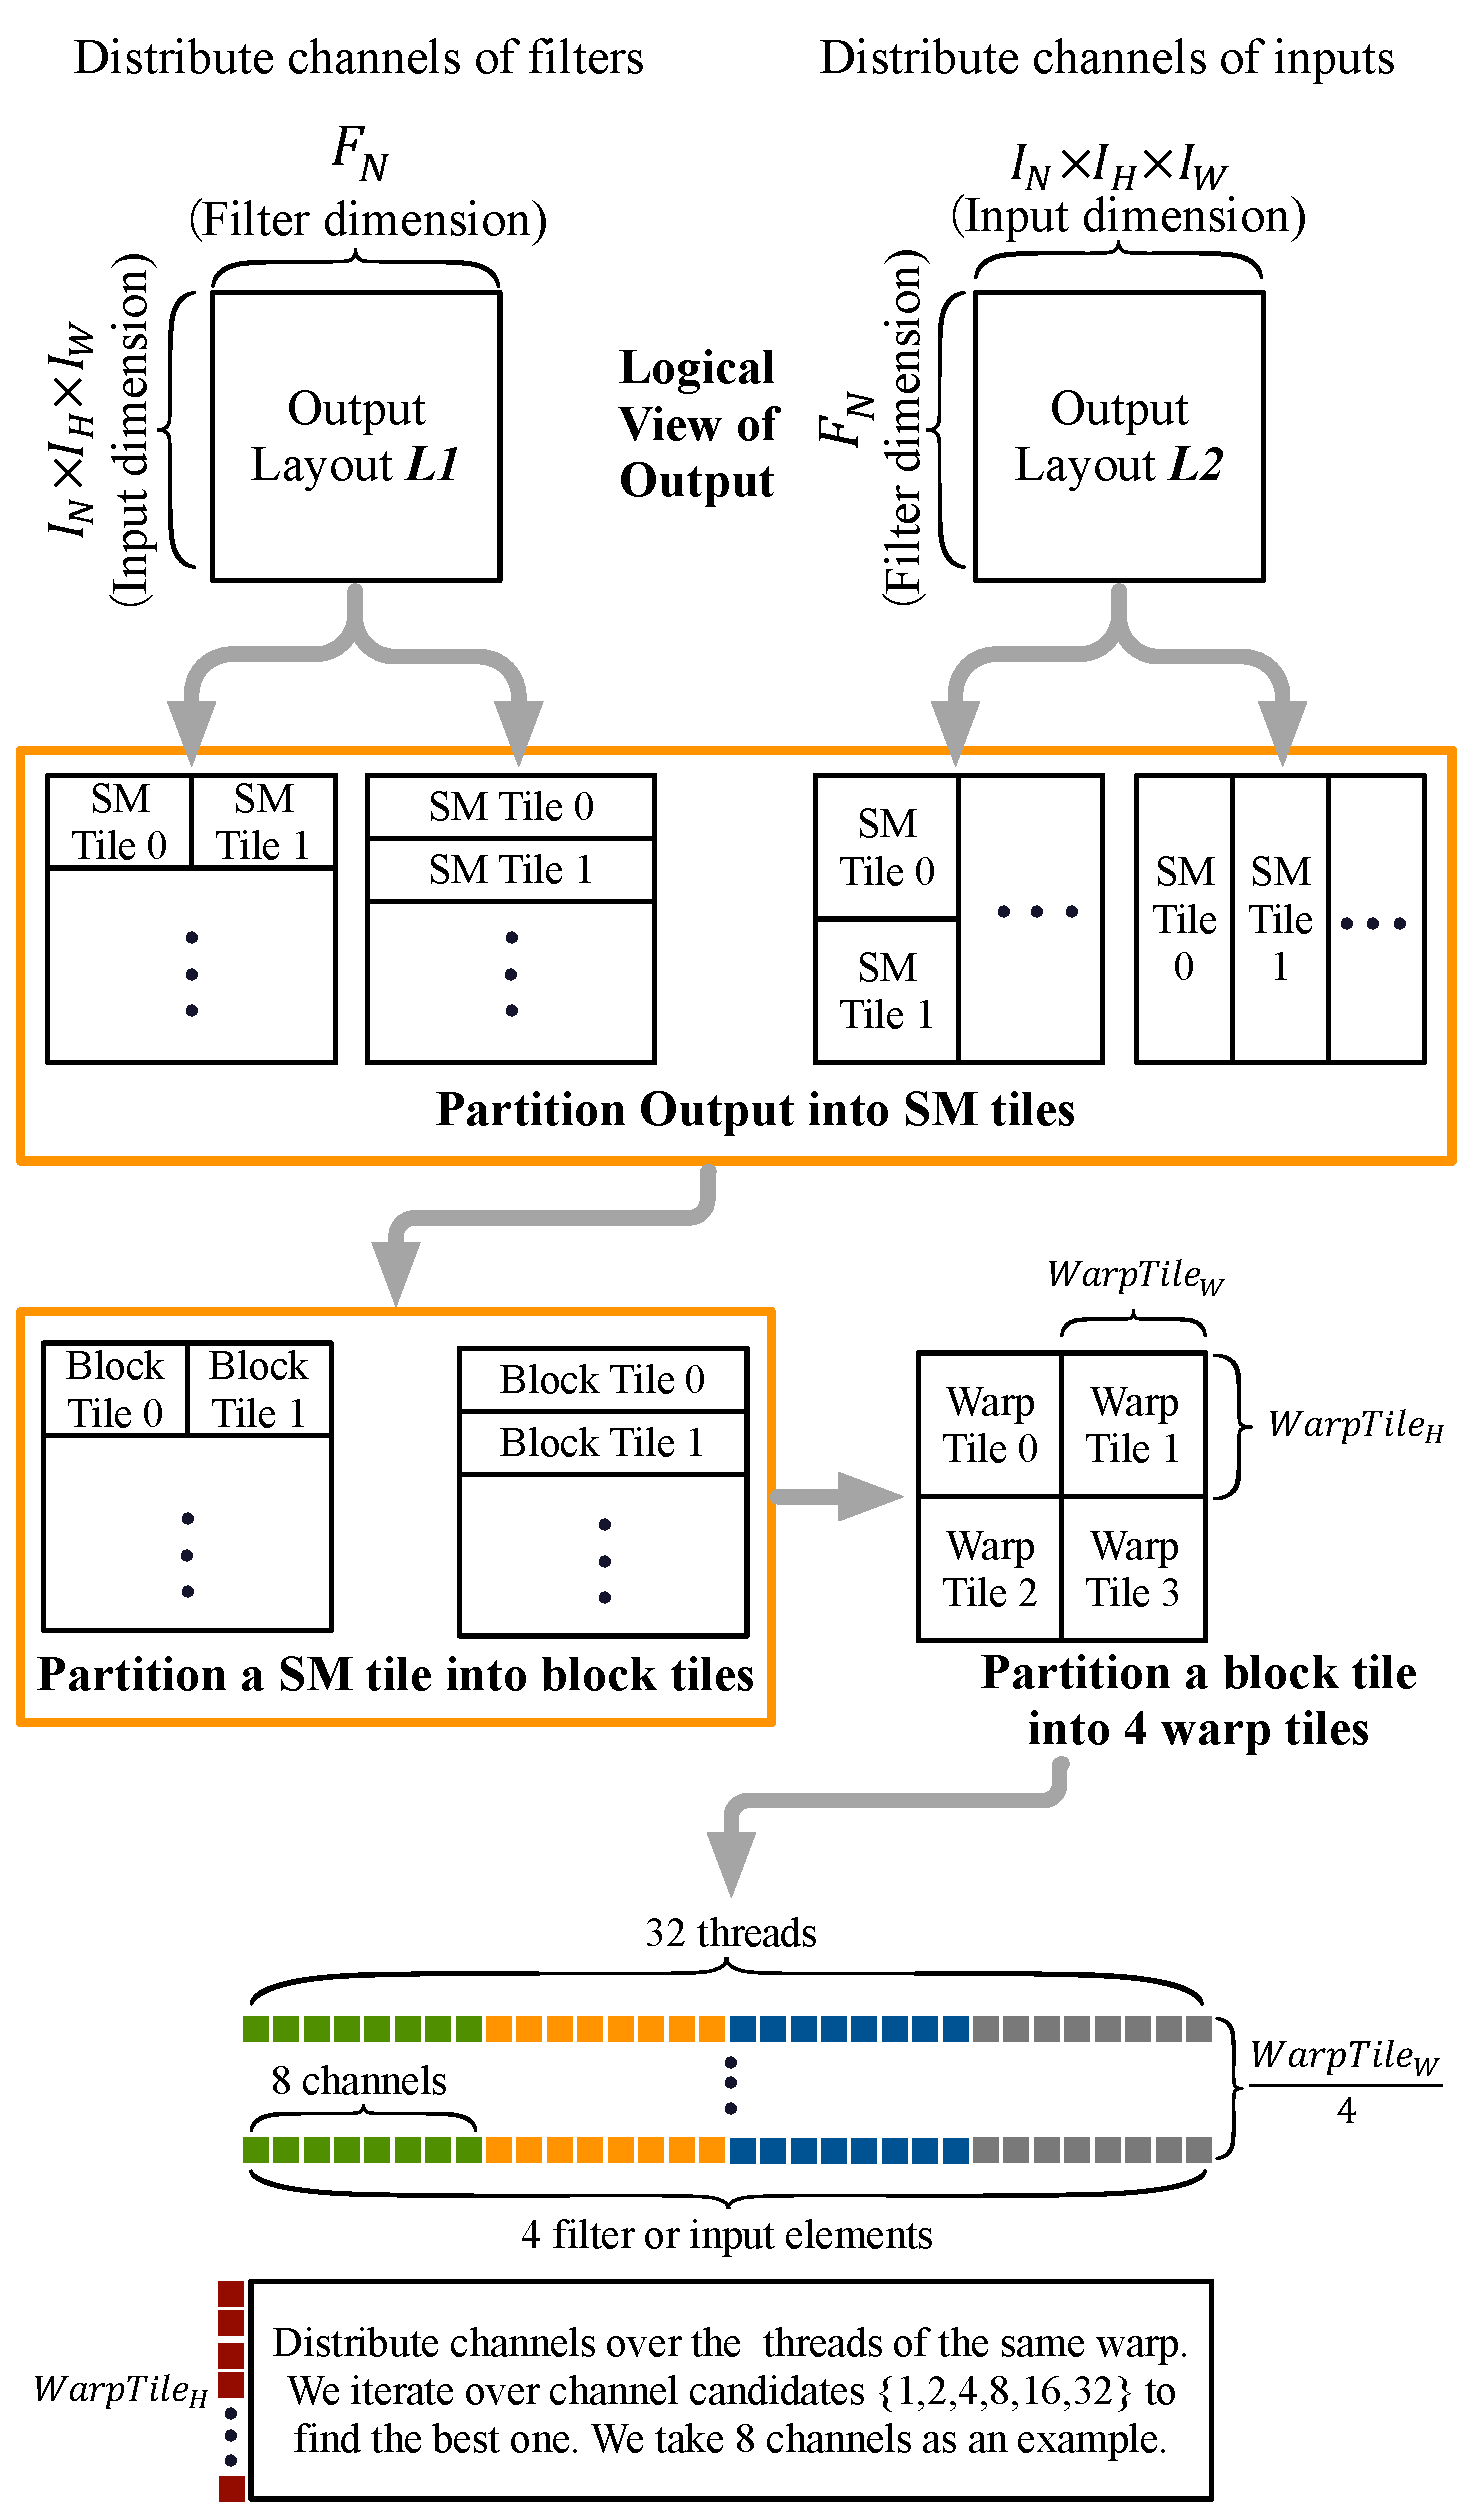
\includegraphics[width=0.95\textwidth,height=7cm]{figure/pwworkflow.eps}
    \vspace{-3mm}
    \caption{Workflow of our 2-level tiling and channel distribution methods.} \label{fig:pwworkflow}
\end{figure*}
\begin{algorithm}[t!]
    \small
        \KwIn{$I$, $F$}
        \KwOut{$O$}
        \tcp{below codes are executed on CPU}
        Determine candidates for relevant parameters\;
        \ForEach{parameter combination}{
            \If{not satisfy constraints of Formula \ref{fo:limitr} and \ref{fo:limits}}{
                continue\;
            }
            Calculate $SM_{util}$ and $AI$ with Formula \ref{fo:smutil} and \ref{fo:diff}\;
            Choose combinations whose $SM_{util}$ is close to 1\;
            Among chosen combinations, choose the combination with the maximal $AI$\;
        }

        Choose the kernel based on the chosen combination.\;
        \tcp{below codes are executed on GPU}
        Load $C_{num}$ channels of a block tile into shared memory array $sharedBuf1$\;
        $\_\_syncthreads()$\;
        \For{$iter \gets 0$ \KwTo $I_C$ By $2 \times C_{num}$}{
            Load next $C_{num}$ channels into $R_{tmp}$\;
            Load channels from $sharedBuf1$ into $R_{operand}$\;
            Accumulate output elements into $R_{result}$\;
            Write $R_{tmp}$ into $sharedBuf2$\;
            $\_\_syncthreads()$\;
            Repeat above steps but swap $sharedBuf1$ and $sharedBuf2$\;
        }
        Use segmented parallel reduction to get the final output elements and write the result to $O$\;
        \caption{Optimized Pointwise Convolution}
        \label{algo:pwalgo}
\end{algorithm}
\subsubsection{Searching workflow}
To guide the search for the optimal combination of parameters, we use two metrics named SM utilization ($SM_{util}$) and arithmetic intensity ($AI$).
Two metrics can be calculated as follows:
\begin{equation}\nonumber
    Block_{count}=\frac{F_N}{2 \times Warp_W} \times \frac{I_N \times I_H \times I_W}{2 \times Warp_H}
\end{equation}
\begin{equation}
    SM_{util}=\frac{Block_{count}}{Block_{num}\times SM_{num}}
    \label{fo:smutil}
\end{equation}
\begin{equation}
    AI = \frac{Warp_H \times T_{num}}{Warp_H+T_{num}}
    \label{fo:diff}
\end{equation}
where $Block_{count}$ is the number of generated thread blocks, $SM_{num}$ is the number of SMs on a GPU. For RTX 2080Ti and Jetson AGX Xavier, $SM_{num}=68$ and $SM_{num}=8$ respectively.

The whole workflow is described in Algorithm \ref{algo:pwalgo}.
We first determine candidates for relevant parameters, including $Warp_H$, $Warp_W$, $Warp_{num}$, $Block_{num}$ and $C_{num}$, based on the size of the input and filter (Line 1).
Then we iterate over all combinations of parameters (Line 2), and keep the combinations that satisfy the constraints $Limit_R$ (Formula \ref{fo:limitr}) and $Limit_S$ (Formula \ref{fo:limits}) (Line 3).

Next, we calculate values of $SM_{util}$ (Formula \ref{fo:smutil}) and $AI$ (Formula \ref{fo:diff}) for all satisfied combinations (Line 5) and select the optimal combination with following steps (Line 6-7):
\begin{enumerate}[Step 1]
    \item If $SM_{util} \geq 1$ is true for all combinations, we select the combinations that possess the smallest and close to the smallest $SM_{util}$.
    The reason is that when $SM_{util} \geq 1$, all SMs are utilized, in which case we want to reduce the number of thread blocks to reduce the number of loads of shared filters or inputs between multiple thread blocks.
    \item If there exists combinations such that $SM_{util}<1$, we first collect these combinations. Then, among collected combinations, we select the ones that possess the biggest and close to the biggest $SM_{util}$.
    The reason is that when $SM_{util}<1$, there are idle SMs, in which case we want to increase $SM_{util}$ to fully utilize SMs. We do not want $SM_{util}$ to exceed 1 because that will incur more memory operations.
    \item Among candidate combinations selected in Step 1 and Step 2, we select the combination with the maximum value of $AI$ because higher arithmetic intensity can hide more global memory access latency.
\end{enumerate}

Last, we choose the pointwise convolution kernel based on the selected combination (Line 8).
In this kernel, each thread block first loads $C_{num}$ channels of the corresponding block tile into shared memory array $sharedBuf1$(Line 9).
Meanwhile, the thread block loads the next $C_{num}$ channels of the block tile into temporary registers (Line 12).
Then, we load data from $sharedBuf1$ into registers (Line 13) and accumulate output elements into registers (Line 14).
Next, we write data in temporary registers into $sharedBuf2$ (Line 15).
The kernel repeats the process until all channels have been accumulated to output elements.
Finally, we use a warp level segmented parallel reduction to reduce results of different channels into the final result and write results to global memory (Line 18).
